\chapter{Metodología}

En este capítulo describimos en profundidad todos los pasos seguidos en los métodos empleados en el trabajo y su justificación. Posteriormente, se aplicarán en la experimentación.

\section{Análisis de los recursos disponibles}

Para la realización de este trabajo debemos considerar los recursos hardware disponibles para la inferencia de los modelos pero sobre todo para el entrenamiento de los modelos.

\begin{enumerate}
	\item \textbf{Hardware en entrenamiento}. Para el desarrollo de toda la experimentación, entrenamiento de los modelos y validación nos valdremos de los recursos que gratuitamente ofrece Kaggle, una plataforma de ciencia de datos propiedad de Google. 
	
	El recurso más importante que ofrece Kaggle y razón de su uso es que nos permite el uso de su gráfica NVIDIA Tesla P100 por 30 horas semanales. Con ella, podemos entrenar los modelos y hacer una inferencia rápida para validación en tiempo razonable.
	
	Los recursos locales que dispongo son un ordenador personal que aunque con mejor capacidad de memoria en disco $\approx 2\ TB$ que la ofrecida por Kaggle $\approx 100\ GB$, nuestra gráfica NVIDIA GeForce RTX 2060 tiene inmensamente menores prestaciones que la ofrecida en Kaggle. A continuación, mostramos una gráfica de rendimiento sobre las características de ambos dispositivos para cuantificar este hecho.
	
	\begin{figure}[H]
		\centering
		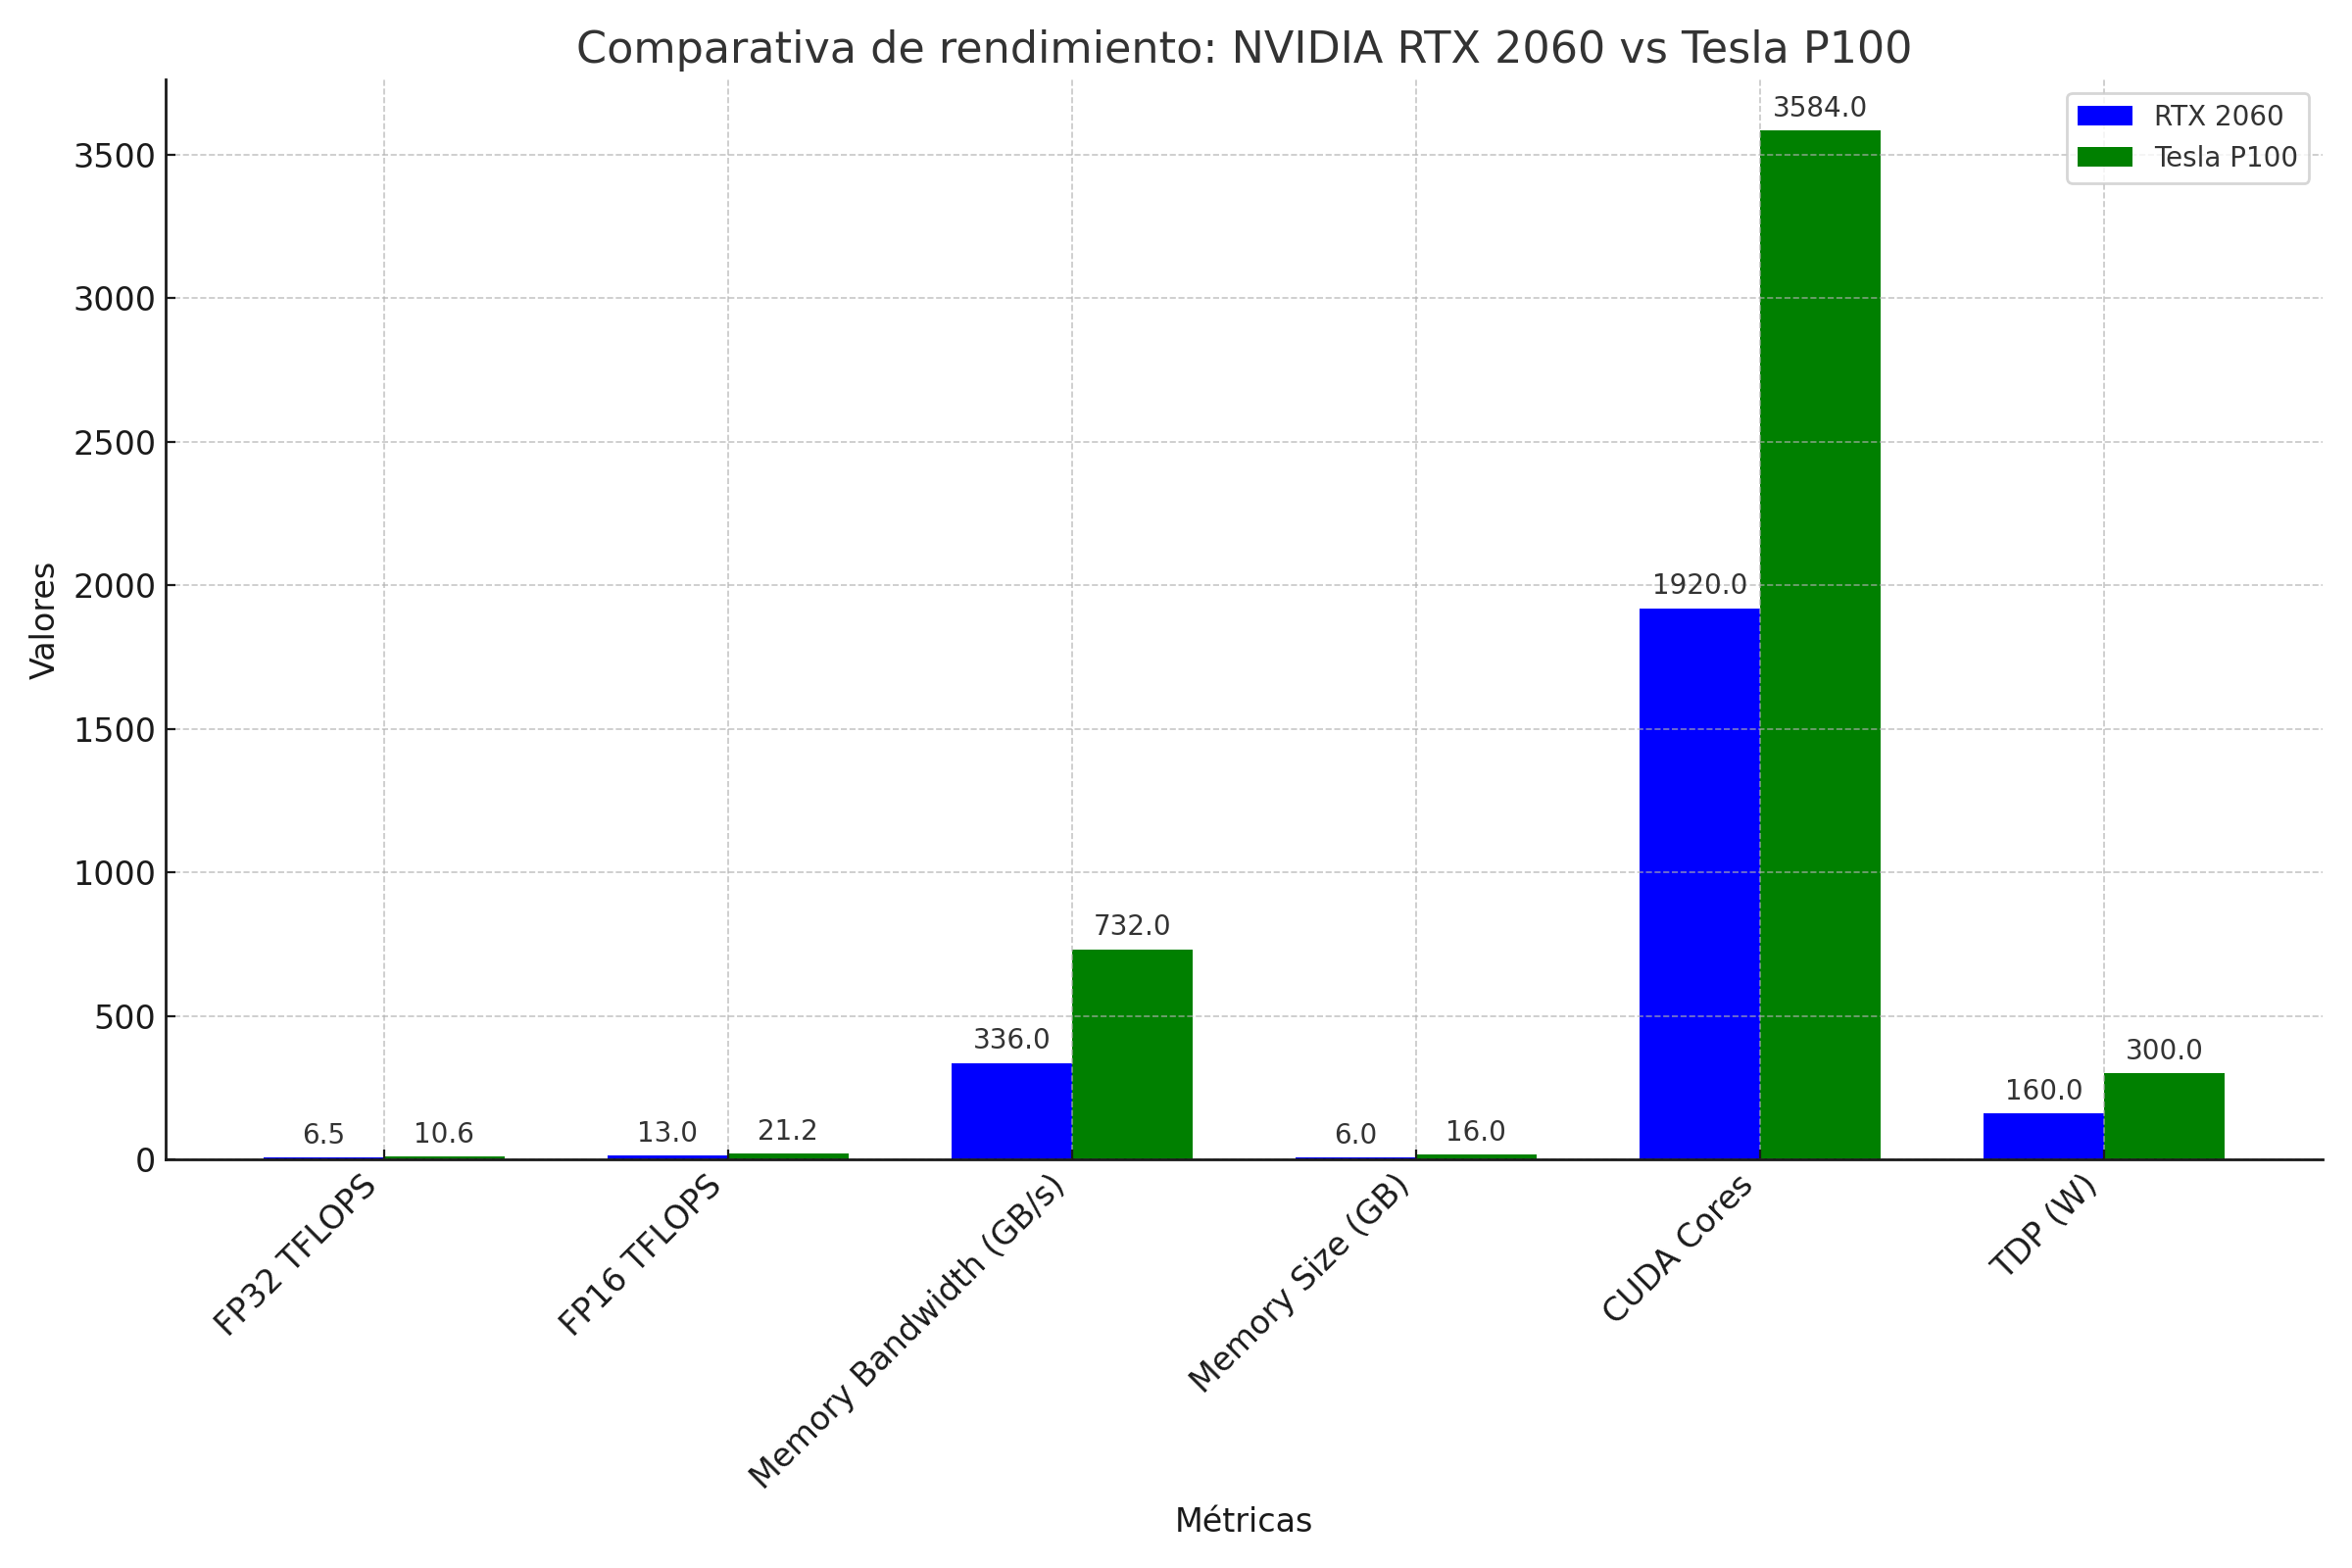
\includegraphics[width=1.0\linewidth]{imagenes/comparativa_rtx2060tesla.png}
		\caption{Comparativa de rendimiento de las GPU disponibles}
	\end{figure}
	
	En todas las características la gráfica ofrecida por Kaggle supera a la nuestra. Por lo que optaremos por usarla en todo el trabajo.
	
	\item \textbf{Hardware para inferir con los modelos}. Para la construcción de la interfaz y su uso si hemos usado nuestro dispositivo personal.
	
	De forma general, el hardware necesario para inferir con los modelos es cualquier PC de uso personal que disponga de una GPU de rendimiento similar o mejor que el nuestro y cumpla las siguientes dependencias (link a apéndice de uso del programa). 
	
\end{enumerate}


\section{Preprocesado de Datos}

En este apartado se explicará el preprocesamiento que se ha aplicado a las resonancias magnéticas para convertirlas a entradas de los modelos. 

Partiendo de nuestro conjunto de datos que presentamos en la introducción obtenido de la competición \textbf{BraTS} en Synapse. Ya vemos como las resonancias presentan características favorables para ser una entrada a la red.

\begin{enumerate}
	\item \textbf{Dimensiones estandarizadas} : Todas las resonancias (adultos, niños, diferente tipo de tumor) presentan las mismas dimensiones.
	\item \textbf{Imágenes estandarizadas} : Todas las resonancias se han hecho con el mismo estándar de escáner, todas presentan el mismo rango para su visualización. 
	\item \textbf{No existen valores faltantes} : Observamos como el conjunto de datos es completo en su definición, todas las resonancias de cada paciente tienen las mismas cuatro pruebas.
\end{enumerate}

\subsection{Elección de dimensionalidad de las entradas}

Una de las elecciones cruciales al inicio del trabajo es la dimensionalidad de las entradas de la red (determina la forma en la que se procesan los datos). ¿Es mejor trabajar en 2D con una única imagen como entrada o en 3D con todo el conjunto de imágenes de una resonancia como entrada?

En un primer momento debido a que la mayoría de literatura actual trabaja en 3D, intentamos trabajar en 3D. Para ello, construimos un primer modelo inicial de arquitectura para 2D y  una forma de transformarlo a 3D es simplemente duplicar cada capa por la cantidad de imágenes en cada resonancia. Por lo que, el tamaño de nuestro modelo inicial 2D $SIZE_{2D}$ sólo debíamos multiplicarlo por la cantidad de imágenes en una resonancia $SIZE_{3D} = SIZE_{2D} \times 155 $. Debido que el máximo de memoria RAM que disponíamos en la Tesla P100 de Kaggle es $16\ GB$ siguiendo esa regla, el máximo tamaño que podría ocupar un modelo inicial 2D sería: 

$$ MAXSIZE_{2D} = \frac{16\ GB}{155}  = 0.10323\ GB = 105.7\ MB $$  

Esta cantidad de memoria para una arquitectura que obtenga resultados competentes en la actualidad de técnicas que existen no es viable. Viéndonos obligados ante la escasez de memoria en GPU a enfocar nuestros esfuerzos en una dimensionalidad 2D. Tendremos como entrada a las arquitecturas \textbf{una única imagen la correspondiente a la vista axial de las resonancias}.

\subsection{Normalizado de las imágenes}

Las imágenes que componen las resonancias son mapas en escala de gris donde un píxel de la imagen puede tomar un valor de gris en el intervalo $[0, 256)$. Entre las imágenes de distintas resonancias se encuentra una misma distribución de valores de píxeles para representar la misma información. Sin embargo, el proceso de entrenamiento no deja de ser un proceso de optimización y puede que este rango sea aún demasiado grande.

Adicionalmente, para evitar posibles píxeles erróneos en la toma de las imágenes que podamos interpretar como outliers que tengan un impacto negativo en el entrenamiento y para hacer las imágenes más interpretables se aplica a las imágenes normalización Z-score o estandarización.

$$ X_{std}^{i}= \frac{x^{i}-mean}{std} $$



\subsection{Recortado de imagen}

Podría ser razonable reducir las dimensiones de las imágenes para hacer que los datos sean menos pesados. Sin embargo, se opta por no hacerlo por seguridad y escalibilidad. \textbf{BraTS} fija esas dimensiones en base al estándar en una resonancia magnética, así para cualquier paciente se garantiza que la imagen de su cerebro se puede representar en una resonancia en unas condiciones de resolución iguales al resto de pacientes.

Si recortamos las imágenes de forma cuadrada al cerebro más grande de todas las resonancias, podríamos encontrarnos en inferencia con un cerebro mayor que no se podría representar en una imagen. Es necesario dejar cierto margen, optando por respetar el margen inicial que marcan los organizadores médicos de \textbf{BraTS}.

\subsection{Undersampling}

En el estado del arte ya mencionamos que existía un desbalanceo entre tejido sano y tejido enfermo. En la mayoría de resonancias existe una mayor proporción de tejido sano que de tejido enfermo. Esto no sólo podía introducir un sesgo en los algoritmos de segmentación sino que aumenta mucho el coste computacional de entrenar a los modelos por el exceso de imágenes que no contienen la información de una lesión tumoral. 

El tratamiento del desbalanceo mediante undersampling siempre es una medida agresiva ya que podría eliminar información que a priori no consideramos relevante y si lo es.

Sin embargo, en nuestro problema aplicaremos undersampling con el principal objetivo de reducir los tiempos de entrenamiento y poder tener una arquitectura más profunda manteniendo tiempos razonables. Intentando aliviar de paso el problema del desbalanceo.
A continuación explicamos en detalle como se ha llevado a cabo.

Para todo nuestro conjunto de datos $X$ creamos archivos CSV para cada partición (entrenamiento, validación y test) donde cada fila de cada archivo CSV representa a una imagen o entrada a la red. 

Estos archivos en formato CSV contendrán únicamente el conjunto de imágenes que contienen lesión tumoral de todas las resonancias $N$ más una parte seleccionada aleatoriamente de imágenes sin lesión de tamaño $\frac{|N|}{2}$. De esta forma, nos quedamos con todas las imágenes con información de lesión y con una parte representativa y balanceada sin lesión para no sesgar al modelo a segmentar en todas las imágenes.

Este es el pseudo-código de creación de los archivos CSV para este proceso de undersampling. 

\begin{algorithm}
	\caption{Undersampling de las imágenes a usar}
	\begin{algorithmic}[1]
		\STATE \textbf{Entrada:} \textit{mri\_paths}, \textit{name}
		\STATE \textbf{Salida:} Archivo CSV con columnas (t1c, t1n, t2f, t2w, slice, etiqueta)
		\STATE \textbf{Inicializar} lista vacía \textit{data}
		
		\FOR{cada \textit{mri\_path} en \textit{mri\_paths}}
		\STATE \textit{label\_path} $\gets$ \textit{mri\_path[1]}
		\STATE \textit{label\_img} $\gets$ Cargar \textit{label\_path}
		\FOR{\textit{slice\_num} en rango(5, 150)}
		\IF{hay algún tumor en \textit{label\_img[:, :, slice\_num]}}
		\STATE \textit{label} $\gets$ 0 si "MEN" $\in$ \textit{label\_path}, sino 1
		\STATE Añadir \{t1c, t1n, t2f, t2w, slice, etiqueta\} a \textit{data}
		\ENDIF
		\ENDFOR
		\STATE Liberar \textit{label\_img} y recolectar basura
		\ENDFOR
		
		\STATE \textit{notumores\_size} $\gets$ longitud de \textit{data} dividido 2
		\FOR{cada $i$ en rango(0, \textit{notumores\_size})}
		\STATE \textit{slice\_num} $\gets$ número aleatorio entre 5 y 150
		\STATE \textit{idx} $\gets$ índice aleatorio entre 0 y longitud de \textit{mri\_paths} - 1
		\IF{el slice y los paths no están en \textit{data}}
		\STATE Añadir \{t1c, t1n, t2f, t2w, slice, etiqueta\} a \textit{data} con \textit{etiqueta} = 2
		\ENDIF
		\ENDFOR
		
		\STATE Convertir \textit{data} a DataFrame \textit{df}
		\STATE Guardar \textit{df} como archivo CSV con nombre \textit{name}
		
	\end{algorithmic}
\end{algorithm}


En estos archivos CSV existen las siguientes columnas:

\begin{enumerate}
	\item \textbf{Rutas absolutas} : En $4$ columnas están las rutas absolutas a los archivos .nii de cada prueba de cada resonancia.
	\item \textbf{Número de slice} : Se guarda el número de slice en la que se localiza esa imagen dentro de la resonancia. Este campo es necesario para poder extraer la imagen.
	\item \textbf{Etiqueta} : Para el problema de clasificación es necesario guardar la etiqueta que identifica a cada imagen, 0 para Meningioma, 1 para Glioblastoma y 2 para No Tumor.
\end{enumerate}

Tras aplicar este undersampling nos quedamos con $74487$ imágenes reducidas $I_{RED}$ en entrenamiento, $31899$ en validación y $45354$ en test respecto a un total de imágenes $I_{TOTAL} = Pacientes \times Slices$. En la siguiente tabla podemos ver recogida esta información también en términos de porcentaje.

\begin{table}[H]
	\centering
	\begin{tabular}{cccc}
		\hline
		\toprule
		\textbf{Partición} & \textbf{$I_{TOTAL}$} & \textbf{$I_{RED}$} & \textbf{Porcentaje $\%$} \\ 
		\midrule
		Entrenamiento & 1033 $\times$ 155 & 74487 &  46.52 \\ 
		Validación & 442 $\times$ 155 & 31899 & 46.56 \\ 
		Test & 632 $\times$ 155 & 45354 &  46.3\\ 
		\bottomrule
	\end{tabular}
	\caption{Porcentaje de imágenes conservadas tras undersampling.}
\end{table}


\section{Elección de modelos}

A continuación pasamos a discutir los modelos y técnicas empleadas para la creación de las arquitecturas. En este trabajo como al igual que en parte del estado del arte combinaremos técnicas de aprendizaje no supervisado y supervisado.

\subsection{Codificador y representación latente}

Ponemos ahora el foco en un modelo en principio pensado para el aprendizaje sin etiquetas, los \textbf{autoencoders}.

Los autoencoders son arquitecturas encoder-decoder con la finalidad de aprender las características de un conjunto de datos o distribución. Por ejemplo, siendo esto útil para obtener modelos generativos como los autoencoders variacionales. 

Los autoencoders se formularon inicialmente como una generalización no lineal del análisis de componentes principales (PCA) por su poder para reducir la dimensionalidad. En este trabajo lo incluiremos como modelo base para aplicar aprendizaje no supervisado y que teóricamente presentarían notables ventajas de cara obtener una mayor convergencia y generalización en el proceso de entrenamiento. 

A continuación, mostramos un esquema explicativo de las partes implicadas en la arquitectura para la reconstrucción de las imágenes necesaria para el construir el codificador y representación latente.

\begin{figure}[H]
	\centering
	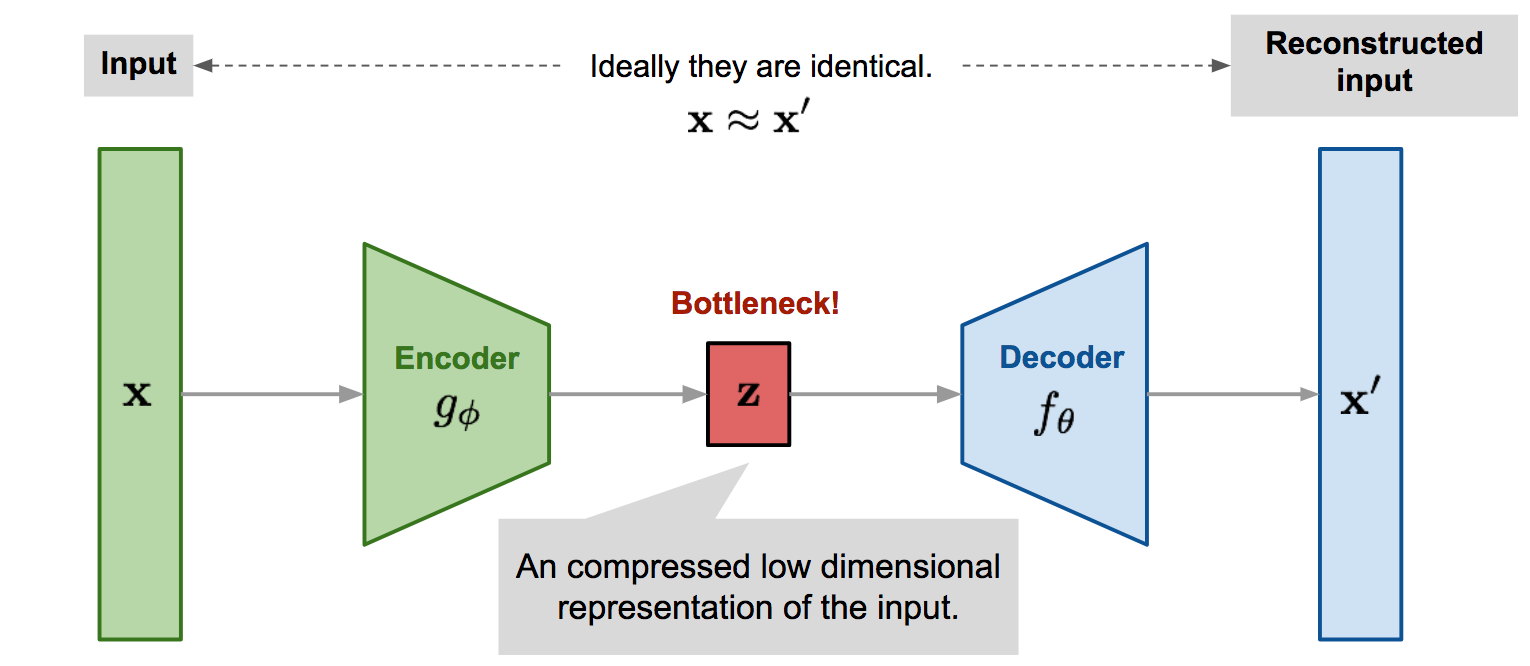
\includegraphics[width=1.0\linewidth]{imagenes/esquema_codificador.png}
	\caption{Esquema de la arquitectura empleada para inicializar el codificador y representación latente. \cite{subedi2022retracted}}
\end{figure}


El objetivo tras aplicar este esquema es construir un fuerte codificador que reduzca la dimensionalidad y una representación latente (bottleneck) que comprima las características principales de las imágenes del conjunto de entrenamiento.

En términos del proceso de optimización que es el entrenamiento, de forma no supervisada se están inicializando los pesos de la red para parecerse al conjunto de imágenes. \cite{zeiler2014visualizing} estudia como los diferentes filtros de las redes neuronales convolucionales al entrenarse ante una tarea de clasificación acaban replicando las características generales y específicas de las imágenes de las que son entrenados. Por ello, se llega a la conclusión de que una heurística importante dentro de las redes neuronales convolucionales es que \textbf{los filtros se parecen a las imágenes}. 

Esta razón explica de forma teórica como un proceso de ajuste previo al conjunto de entrenamiento elimina el coste computacional de búsqueda de los pesos via descenso del gradiente y backpropagation que require el ajuste de la red por sí misma a las imágenes sólo a partir de las etiquetas.

\subsection{Modelo de clasificación}

A continuación, presentamos el modelo de clasificación.

La entrada $x$ es el vector de características iniciales. En nuestro caso, son las tres imágenes correspondientes a las $3$ pruebas. El codificador es una red neuronal que transforma la entrada de alta dimensionalidad $x$ en una representación de menor dimensionalidad $z$. El proceso de codificación se puede ver como una función $g_{\phi}$ parametrizada por $\phi$, que aprende a extraer las características más relevantes de los datos de entrada. La parte final del esquema es una red neuronal densa que toma la representación comprimida $z$ y realiza la tarea específica del modelo

\begin{figure}[H]
	\centering
	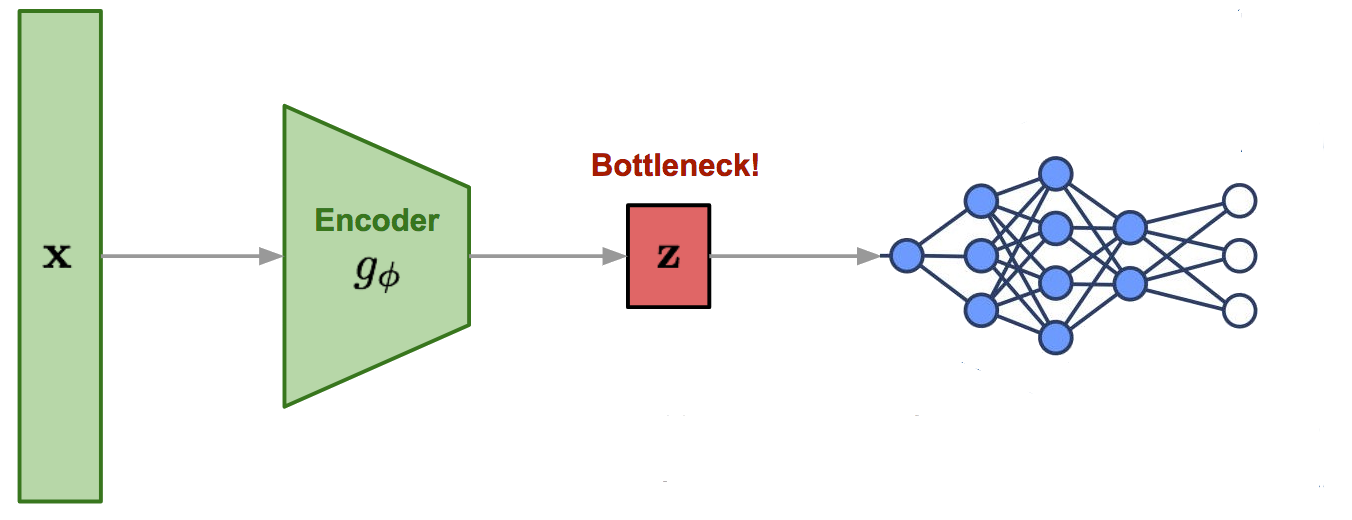
\includegraphics[width=0.9\linewidth]{imagenes/esquema_clasificacion.png}
	\caption{Esquema de la arquitectura empleada para el problema de clasificación}
\end{figure}

Tras ello tenemos un modelo capaz de distinguir entre las etiquetas \textbf{glioblastomas, meningiomas o no tumor} para imágenes donde aparecer uno de los esos dos tumores o no aparezca ninguno. Para transformarlo en un clasificación binaria para todas las imágenes de una resonancia aplicamos el siguiente esquema de votación.

\subsubsection{Esquema de votación}

Tras la salida de las neuronas en las $3$ etiquetas creadas para trabajar en 2D: \textbf{glioblastomas, meningiomas o no tumor}. Necesitamos una transformación de las predicciones individuales de cada imágenes a toda la resonancia. En la mayoría de los casos ante este tipo de problema se usa un \textbf{esquema de votación}.

Consideraremos un esquema de votación que utilice solo la cantidad de predicciones cuando exista tumor, es decir, cuando la etiqueta sea \textbf{Glioblastoma} o \textbf{Meningioma}. Mostraremos el esquema de votación que usamos en el siguiente pseudo-código.

\begin{algorithm}
	\caption{Predicción del tipo de tumor de toda la resonancia a partir de las predicciones de todas las imágenes de este}
	\begin{algorithmic}[1]
		\STATE \textbf{Function} \texttt{Votación}($Meningioma_{PREDS}$, threshold)
		\IF{$Meningioma_{PREDS} < threshold$}
		\STATE \textbf{return} "Meningioma"
		\ELSE
		\STATE \textbf{return} "Glioblastoma"
		\ENDIF
	\end{algorithmic}
\end{algorithm}

Tras este método sólo queda saber cual es el parámetro $threshold$ óptimo. Para ello, simplemente se ajustará a validación tras una búsqueda a través de fuerza bruta.

\subsection{Modelo de segmentación}

A continuación, presentamos el modelo para la tarea de segmentación. Muy similar al esquema para la reconstrucción tenemos un diferente y totalmente nuevo decodificador $S_{\sigma}$ especifico para la tarea de crear una máscara de segmentación. Se añaden conexiones (concatenaciones) entre el codificador y decodificador para poder preservar la precisión de las características de la imagen original. Finalmente la salida son las etiquetas $Y$ las cuales son las máscaras segmentación reales proporcionadas por \textbf{BraTS} y umbralizadas a toda la lesión tumoral.


\begin{figure}[H]
	\centering
	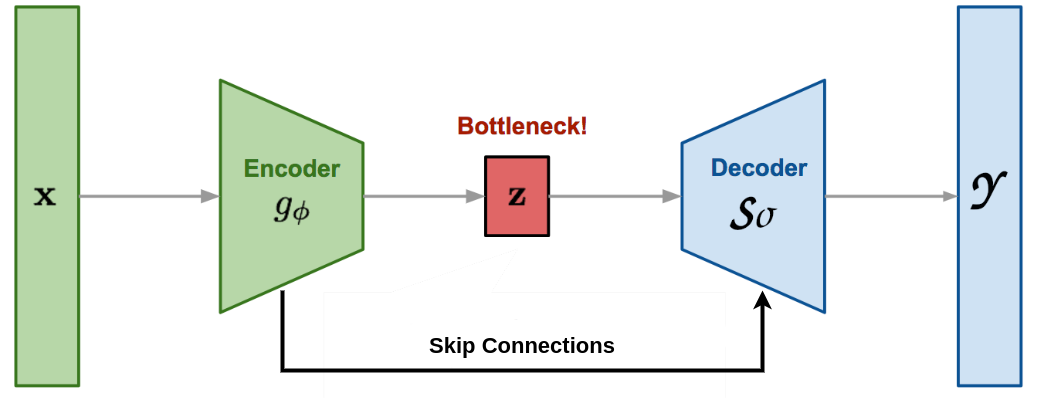
\includegraphics[width=0.9\linewidth]{imagenes/esquema_segmentacion.png}
	\caption{Esquema de la arquitectura empleada para el problema de segmentación}
\end{figure}

\subsection{Uso de transfer learning}

Dentro de las estrategias que podemos utilizar para una mayor convergencia en el aprendizaje y disminuir los tiempos de entrenamiento incluiremos el uso de \textbf{transfer learning}.

Debemos tener en cuenta que el entrenamiento en la tarea de la reconstrucción de las imágenes también es una estrategia de transfer learning, ya que transferimos el aprendizaje útil de la tarea de la reconstrucción a las tareas específicas del problema. Sin embargo, en esta sección nos enfocamos en usar transfer learning previamente a esa tarea. 

La única parte que usaremos de la arquitectura usada en el autoencoder será el codificador por tanto sólo nos preocupa el uso de transfer learning en esa parte de la red. En la búsqueda de un buen codificador $g_{\phi}$ podemos encontrar arquitecturas usadas en clasificación que capturan características visuales generales, de millones de imágenes diferentes. Es común para multitud de problemas el uso de arquitecturas previas entrenadas con el dataset \textbf{ImageNet}. 

Optamos por tomar como codificador una arquitectura previamente entrenada en este dataset, las arquitecturas candidatas que probaremos en el desempeño del problema serán: 

\begin{enumerate}
	\item \textbf{ResNet34}: Por su multitud de conexiones residuales reportadas en el estado del arte como factor positivo. Con una profundidad de 34 capas está entre sus arquitecturas hermanas ResNet18 y ResNet50 como una arquitectura no muy profunda que ofrece buen desempeño para variedad de problemas.
	
	\item \textbf{Xception}: A diferencia de \textbf{ResNet34} ofrece kernels de distinto tamaño que podrían favorecer la mejor caracterización de tumores de diferente tamaño. 
	
\end{enumerate}


\section{Diseño de las arquitecturas}

En el siguiente apartado detallaremos los módulos y capas que componen a las arquitecturas así como las componentes importantes. 

\subsection{Función de activación}

Para todas las arquitecturas (segmentación, clasificación y el autoencoder para construir el codificador), se optará por el uso de la función de activación ReLU (Rectified Linear Unit), definida como:

$$ \text{ReLU}(x) = \max(0, x) $$

Donde \( x \) es la entrada a la función ReLU.

A continuación, enunciamos algunas de las razones de su elección y su reconocida robustez para una gran amplitud de problemas en aprendizaje profundo.

\begin{enumerate}
	\item \textbf{No Linealidad:}
	ReLU introduce no linealidad en las redes neuronales, lo cual es crucial para que las redes puedan aprender y modelar relaciones y características complejas en los datos. Esta no linealidad es esencial para tareas como la clasificación y la segmentación, donde las relaciones entre los datos son inherentemente no lineales.
	
	\item \textbf{Gradiente Constante:}
	Para valores positivos de $ x $, la derivada de ReLU es constante e igual a 1. Esto evita el problema del desvanecimiento del gradiente en redes profundas, donde el gradiente puede volverse extremadamente pequeño en funciones de activación saturadas como la sigmoide y la tangente hiperbólica.
	
	\[ \frac{\partial \text{ReLU}(x)}{\partial x} = \begin{cases} 
		1 & \text{si } x > 0 \\
		0 & \text{si } x \leq 0 
	\end{cases} \]
	
	Esto facilita el entrenamiento de redes más profundas y la convergencia más rápida durante el proceso de optimización.
	
	\item \textbf{Eficiencia Computacional:}
	La función ReLU es eficiente en términos computacionales. Su implementación es simple (una comparación y una operación de máximo) y no involucra cálculos costosos como funciones exponenciales.
	
\end{enumerate}

La elección de ReLU como función de activación común a través de estas arquitecturas se basa en sus propiedades matemáticas que promueven la eficiencia, la no linealidad y la estabilidad del gradiente.

\subsection{Normalización por lotes}

Antes de aplicar la función de activación, aplicaremos \textbf{normalización por lotes}.
PyTorch que es la biblioteca que usaremos implementa la normalización por lotes descrita en \cite{ioffe2015batch}.

La normalización por lotes se aplica a la salida de una capa antes de aplicar la función de activación. Supongamos que tenemos una capa con activaciones $\mathbf{x}$, donde $\mathbf{x} \in \mathbb{R}^{m \times d}$, siendo $m$ el tamaño del lote y $d$ el número de características en cada ejemplo del lote.

Se calcula la media para cada característica a lo largo del lote:
\[
\mu_j = \frac{1}{m} \sum_{i=1}^{m} x_{ij}
\]
donde $\mu_j$ es la media de la característica $j$ y $x_{ij}$ es el valor de la característica $j$ del ejemplo $i$ en el lote.

Se calcula la varianza para cada característica a lo largo del lote:
\[
\sigma_j^2 = \frac{1}{m} \sum_{i=1}^{m} (x_{ij} - \mu_j)^2
\]
donde $\sigma_j^2$ es la varianza de la característica $j$.


Los datos se normalizan utilizando la media y la varianza calculadas:
\[
\hat{x}_{ij} = \frac{x_{ij} - \mu_j}{\sqrt{\sigma_j^2 + \epsilon}}
\]
donde $\hat{x}_{ij}$ es la característica $j$ del ejemplo $i$ normalizada, y $\epsilon$ es una pequeña constante (generalmente $10^{-5}$) para evitar la división por cero y mejorar la estabilidad numérica.


Después de la normalización, se aplica un escalamiento y un sesgo:
\[
y_{ij} = \gamma_j \hat{x}_{ij} + \beta_j
\]
donde $y_{ij}$ es la salida final para la característica $j$ del ejemplo $i$, $\gamma_j$ es un parámetro de escala aprendido, y $\beta_j$ es un parámetro de sesgo aprendido.

Durante el entrenamiento, tanto $\gamma_j$ como $\beta_j$ se optimizan junto con los otros parámetros de la red neuronal mediante el descenso de gradiente.

El uso de normalización por lotes tiene algunos \textbf{beneficios}.
\begin{itemize}
	\item \textbf{Estabilización del entrenamiento:} La normalización por lotes ayuda a reducir los problemas de desvanecimiento y explosión del gradiente, permitiendo que las redes neuronales más profundas se entrenen de manera más efectiva.
	\item \textbf{Regularización:} Actúa como una forma leve de regularización al introducir una varianza controlada en el proceso de entrenamiento, lo que a menudo conduce a una mejor generalización del modelo.
\end{itemize}


\subsection{Arquitectura para la reconstrucción de imágenes}

Como anunciábamos usamos una arquitectura bien conocida como codificador, probaremos la bondad de \textbf{ResNet34} y \textbf{Xception} en la experimentación. Tras ello, construimos un intuitivo espacio de capas que sean nuestra representación latente. 

\subsubsection{Arquitectura del codificador ResNet34}

A continuación, mostramos y comentamos la arquitectura de uno de los posibles codificadores que usaremos ResNet34.

La innovación clave de ResNet es el bloque residual, que introduce atajos o conexiones directas entre capas no adyacentes de la red. Estos bloques permiten que el flujo de información y los gradientes se propaguen directamente a través de la red, mitigando los problemas de desaparición y explosión del gradiente.

Un bloque residual típico se representa como:
$$ \mathbf{y} = \mathcal{F}(\mathbf{x}, \{W_i\}) + \mathbf{x} $$

Aquí, \(\mathbf{x}\) es la entrada del bloque, \(\mathcal{F}(\mathbf{x}, \{W_i\})\) es la transformación no lineal aprendida (que puede incluir capas como convoluciones, normalización y activaciones), y \(\mathbf{x}\) se suma a esta transformación para obtener la salida \(\mathbf{y}\). Esta suma es la conexión residual.

\begin{figure}[H]
	\centering
	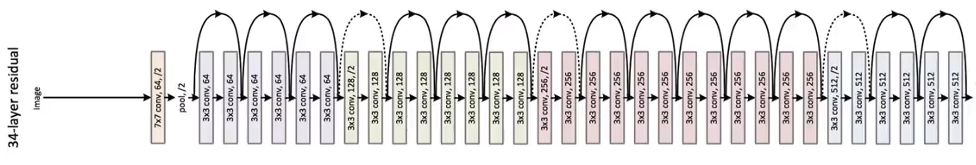
\includegraphics[width=1.0\linewidth]{imagenes/resnet34_arch.png}
	\caption{Arquitectura usada de ResNet34 \cite{he2016deep}}
\end{figure}

ResNet34 se compone de varias capas organizadas en bloques residuales. Como \textbf{capa de entrada} tiene una capa convolucional inicial con 64 filtros de tamaño 7x7 y un stride de 2, seguida de una capa de normalización y una capa de pooling de 3x3 con un stride de 2. Tras ello tenemos los siguientes \textbf{bloques residuales}:
\begin{itemize}
	\item 3 bloques con 64 filtros.
	\item 4 bloques con 128 filtros.
	\item 6 bloques con 256 filtros.
	\item 3 bloques con 512 filtros.
\end{itemize}

Cada bloque está compuesto por dos capas convolucionales de tamaño 3x3. Los bloques están organizados de manera que cada grupo de bloques de un determinado número de filtros tiene el mismo número de filtros a lo largo del grupo.

Como \textbf{capa final} después de todos los bloques residuales, se añade una capa de pooling global seguida de una capa completamente conectada (fully connected) que produce la salida final de la red. En este trabajo eliminamos esas dos capas finales para añadirle la representación latente.

\subsubsection{Arquitectura del codificador Xception}

A continuación, mostramos y comentamos la arquitectura de uno de los posibles codificadores que usaremos, \textbf{Xception}.

La arquitectura Inception, particularmente en sus versiones más recientes como Inception-v3, utiliza módulos Inception para capturar tanto características locales como globales en las imágenes. Sin embargo, estos módulos son complejos y pueden ser optimizados. Xception simplifica y mejora este diseño usando convoluciones separables en profundidad, lo que resulta en una red más eficiente y efectiva.

\begin{figure}[H]
	\centering
	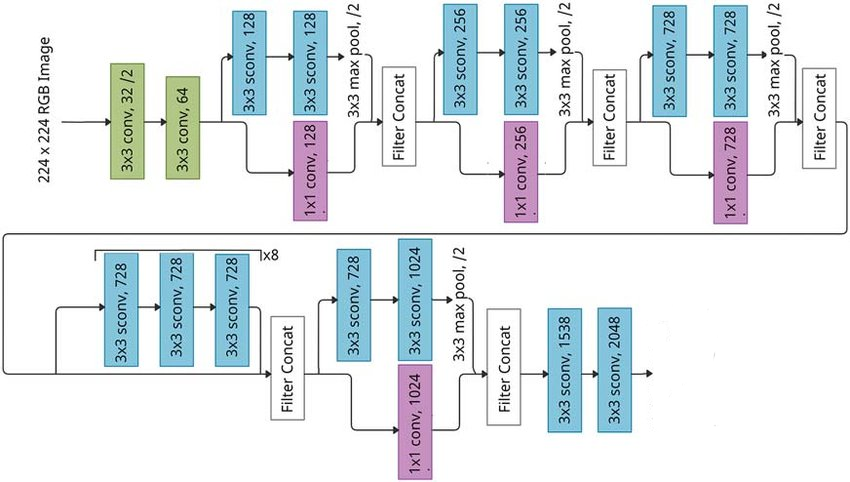
\includegraphics[width=0.8\linewidth]{imagenes/xception_arch.png}
	\caption{Arquitectura usada de Xception \cite{srinivasan2021performance}}
\end{figure}

La convolución separable en profundidad es una técnica que factoriza una convolución estándar en dos operaciones más simples y eficientes: una \textbf{convolución en profundidad} (depthwise convolution) y una \textbf{convolución puntual} (pointwise convolution). En una convolución estándar, los filtros de convolución mezclan canales de entrada y espaciales en una única operación. En cambio, la convolución separable en profundidad realiza estos dos pasos por separado.

Matemáticamente, una convolución separable en profundidad donde \(\mathbf{X}\) es la entrada, \(\mathbf{K}\) es el filtro de convolución, \(*_{\text{depthwise}}\) es la operación de convolución en profundidad y \(*_{\text{pointwise}}\) es la operación de convolución puntual.

Xception se compone de varias capas organizadas en bloques de convolución separables en profundidad. Como capa de entrada tiene una capa convolucional inicial con 32 filtros de tamaño 3x3 y un stride de 2, seguida de una capa convolucional con 64 filtros de tamaño 3x3.

\begin{itemize}
	\item \textbf{Entrada al módulo}: Tres bloques con convoluciones separables en profundidad con 128, 256 y 728 filtros respectivamente.
	\item \textbf{Módulos intermedios}: Ocho bloques idénticos con convoluciones separables en profundidad con 728 filtros cada uno.
	\item \textbf{Salida del módulo}: Tres bloques con convoluciones separables en profundidad con 728, 1024 y 1536/2048 filtros respectivamente.
\end{itemize}

Cada bloque de convolución separable en profundidad consiste en una convolución en profundidad seguida de una convolución puntual y una capa de activación ReLU.

Al igual que \textbf{ResNet34} en la arquitectura original se añade una capa de pooling global seguida de una capa completamente conectada (fully connected) que produce la salida final de la red. Sin embargo, nosotros eliminamos esas capas y le conectamos la representación latente.

\subsubsection{Espacio de capas de la representación latente y bloque ConvBlock}

A continuación, describiremos qué capas y dimensiones tiene la representación latente. Para todas las tareas (clasificación y segmentación) al igual que el codificador se compartirá la misma representación latente. Podemos ver la arquitectura de la representación latente en un diagrama.

\begin{figure}[H]
	\centering
	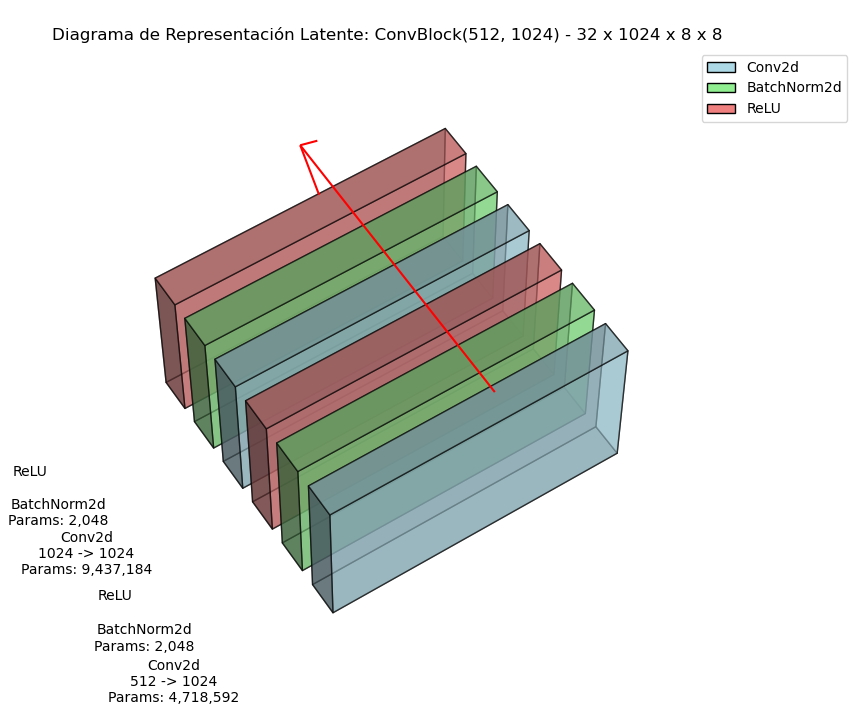
\includegraphics[width=0.8\linewidth]{imagenes/bottleneck_arch.png}
	\caption{Arquitectura de la representación latente}
\end{figure}

El bloque \textbf{ConvBlock(512, 1024)} se utiliza como representación latente dentro de nuestro autoencoder representa una etapa de procesamiento que transforma una entrada de 512 canales (o características) en una salida de 1024 canales mediante operaciones convolucionales seguidas de normalización y activación no lineal. En detalle, el bloque consiste de dos capas convolucionales cada una seguida por capas de Batch Normalization y activación ReLU. La primera capa convolucional transforma los 512 canales de entrada en 1024 canales de salida, manteniendo el tamaño de la entrada con un kernel de 3x3, stride de 1 y padding de 1. Luego, la segunda capa convolucional opera sobre los 1024 canales de salida, manteniendo este número de canales con el mismo tamaño de kernel y configuración de stride y padding. La capa de Batch Normalization se aplica después de cada capa convolucional para estabilizar y acelerar el entrenamiento, y la ReLU como función de activación introduce no linealidades que ayudan a capturar características más complejas en los datos de entrada. Este tipo de bloque que funciona como representación latente del conjunto de datos, es crucial en redes autoencoder para aprender representaciones más profundas y significativas de los datos, condensando y expandiendo la información a través de capas convolucionales apiladas.

\subsubsection{Reducción de canales}

Ambas arquitecturas que probaremos \textbf{ResNet34} y \textbf{Xception} están inicialmente pensadas para imágenes a color, es decir, imágenes en RGB que contenga tres canales o capas pertenecientes a cada tonalidad de colores primarios. Intuitivamente y apoyado por el estado del arte una simple forma de manejar las pruebas para construir una entrada a la red es \textbf{concatenarlas}. De esta forma, una entrada a la red estaría compuesta de una imagen de cuatro canales (uno por tipo resonancia que tenemos o prueba), en otras palabras cuatro imágenes en escala de grises concatenadas respecto un eje $Z$ que representaría la profundidad del volumen de la entrada.


Sin embargo, las arquitecturas empleadas como codificador sólo aceptan imágenes de tres canales. Para lidiar con ello se plantea una reducción de dimensionalidad para transformar las imágenes de cuatro canales a tres canales. A nivel práctico se plantea llevarse a cabo mediante:

\begin{enumerate}
	\item \textbf{Transformación mediante análisis de componentes principales PCA a las tres componentes principales}. Se plantea como la mejor solución de las dos que exploraremos ya que se reduce la información manteniendo la mayor variabilidad posible tras combinar linealmente las imágenes. 
	
	Podemos apreciar como la imagen de una resonancia es transformada con PCA dando la siguiente salida.
	
	\begin{figure}[H]
		\centering
		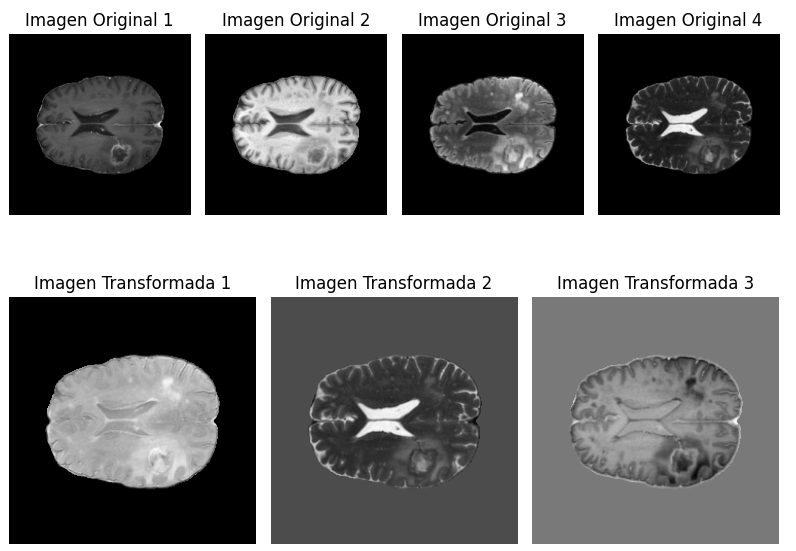
\includegraphics[width=0.8\linewidth]{imagenes/PCA_reduction.png}
		\caption{Ejemplo de transformación mediante PCA}
	\end{figure}
	
	Para aplicar PCA podemos optar por diferentes estrategias atendiendo si queremos incluirlo o no como una más del preprocesamiento de datos.
	
	\begin{enumerate}
		\item \textbf{Mediante el preprocesamiento de todo el conjunto de datos aplicando PCA}. Se puede preprocesar los datos y subirlos a Kaggle de nuevo. Sin embargo, esta opción no se pudo aplicar en la práctica debido a las limitaciones de espacio en disco que nos daba la plataforma.
		
		\item \textbf{Mediante la aplicación de PCA en el mismo entrenamiento antes de introducirlo a la red}. Esta opción elimina la sobrecarga en memoria en disco de Kaggle pero en la práctica es rápidamente descartada ya que aumenta $\approx 50 \%$ el tiempo en entrenamiento. Esta implicación teniendo una limitación de tiempo en Kaggle muy ajustada no la hacen compatible con un entrenamiento completo.
	\end{enumerate}
	
	\item \textbf{Eliminación de una prueba}. Una solución más agresiva es la propia eliminación de un canal de entre los originales. Las principales ventajas de esta solución es la gran facilidad para aplicarla y la mejora del tiempo de extracción de las imágenes puesto ya ahorraríamos traer la eliminada mejorando un $25 \%$ los tiempos de extracción de disco. 
	
	Ante la imposibilidad de aplicar PCA se aplicará esta segunda solución. Se elige eliminar a las imágenes de las resonancias de tipo \textbf{T2W} por ajuste al problema. Se descarta la eliminación de la información con y sin agente de contraste que proporcionan las tipo T1. Entre la elección de \textbf{T2F} y \textbf{T2W} la diferencia principal entre las dos es que en la de tipo \textbf{T2W} el líquido cefalorraquídeo contrasta. En toda la revisión médica del problema no se indica que sea un factor relevante en la segmentación de tumores cerebrales por lo que se conserva a la de tipo \textbf{T2F} que mantiene una imagen más nítida al no contrastar con el líquido cefalorraquídeo.
	
\end{enumerate}

\subsubsection{Bloque UpConv}

Con el objetivo de describir la parte decodificadora de la arquitectura vamos a definir nuestro propio bloque \textbf{UpConv}. Definimos el bloque UpConv como una operación de convolución transpuesta seguido de la aplicación del bloque \textbf{ConvBlock} definido en el apartado de la representación latente.

La \textbf{operación de convolución transpuesta o deconvolución} se define como la inversa de la convolución estándar en una red neuronal convolucional. A continuación, se explica los detalles matemáticos de la convolución transpuesta.

\begin{enumerate}
	\item \textbf{Entrada}: Sea \( x \in \mathbb{R}^{C_{in} \times H_{in} \times W_{in}} \), donde \( C_{in} \) es el número de canales de entrada, y \( H_{in}, W_{in} \) son la altura y anchura de la entrada, respectivamente.
	
	\item \textbf{Salida}: Sea \( y \in \mathbb{R}^{C_{out} \times H_{out} \times W_{out}} \), donde \( C_{out} \) es el número de canales de salida, y \( H_{out}, W_{out} \) son la altura y anchura de la salida, respectivamente.
\end{enumerate}

La operación de convolución transpuesta aplica un kernel de convolución de tamaño \( (k_{H}, k_{W}) \) sobre la entrada \( x \), utilizando un paso (stride) \( s \) y un relleno (padding) \( p \). En nuestro caso, siendo siempre constante $p = 0$ y $s = 2$ La operación se define de la siguiente manera:

\[
H_{out} = (H_{in} - 1) \cdot s - 2p + k_{H}
\]
\[
W_{out} = (W_{in} - 1) \cdot s - 2p + k_{W}
\]

Número de canales de salida: \( C_{out} \)

Sea \( w \in \mathbb{R}^{C_{out} \times C_{in} \times k_{H} \times k_{W}} \) el kernel de la convolución transpuesta.

Para cada posición \( (h', w') \) en la salida:
\[
y_{c}(h', w') = \sum_{c'=1}^{C_{in}} \sum_{h=0}^{k_{H}-1} \sum_{w=0}^{k_{W}-1} w_{c,c',h,w} \cdot x_{c'}(h' \cdot s + h - p, w' \cdot s + w - p)
\]

donde \( y_{c}(h', w') \) es el elemento en la posición \( (h', w') \) del canal \( c \) de la salida \( y \), \( x_{c'} \) es el elemento en la posición correspondiente en el canal \( c' \) de la entrada \( x \), y \( w_{c,c',h,w} \) es el peso del kernel en la posición \( (c, c', h, w) \).

El principal objetivo de la deconvolución es aumentar las dimensiones espaciales de la imagen de entrada, permitiendo reconstruir información espacialmente más detallada a partir de las características aprendidas. De esta forma, el decoder puede reconstruir las imágenes o máscaras a partir de la reducción de las imágenes entrada a la red. 

\subsubsection{Decodificador}

Construimos el decodificador como la secuencia de cuatro bloques \textbf{UpConv}. En este caso, para la primera tarea de reconstrucción con entradas y salidas: (1024, 512), (512, 256), (256, 128), (128, 64). 

\subsection{Arquitectura para clasificación}

Tras la construcción de la arquitectura para reconstrucción ya tendríamos listos el codificador y la representación latente. Para resolver el problema de clasificación creamos la siguiente arquitectura.

\begin{figure}[H]
	\centering
	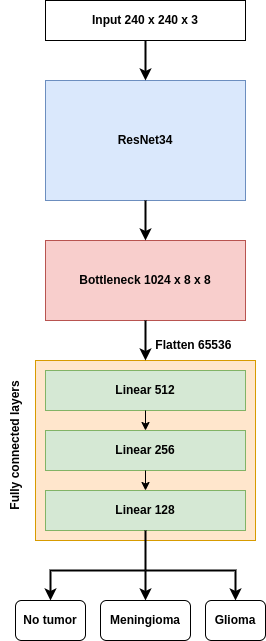
\includegraphics[width=0.3\linewidth]{imagenes/arquitectura_clasificacion.png}
	\caption{Arquitectura para la tarea de clasificación}
\end{figure}

Utilizamos el codificador seguido de la representación latente tras la representación latente aplanamos su salida con una capa \textbf{Flatten} para ahora solo quedará reducir esta salida a $3$ neuronas mediante la aplicación de varias capas de neuronas densamente conectadas. En concreto, $3$ capas con $512$, $256$ y $128$ neuronas hasta la capa final de $3$ neuronas de la que tomamos su máxima neurona como salida.

\subsection{Arquitectura para segmentación}

Tras construir la arquitectura autoencoder para el problema de la reconstrucción, adaptarla para el problema de segmentación es una tarea sencilla. Por un lado, observamos como la estadarización que presentan los datos es favorable para que una misma arquitectura (en el contexto que es una red con unas dimensiones y capas fijas) sea igualmente apta en ambos problemas (reconstrucción y segmentación). Si recordamos \cite{myronenko20193d} utilizaba esta idea, su arquitectura de doble tarea comparte codificador y representación latente, y además ambos decodificadores son prácticamente idénticos. Por lo tanto, se mantendrá el mismo diseño de decodificador que en la tarea de la reconstrucción. La única diferencia que se introducirá en segmentación será el uso de \textbf{skips connections}.

\subsubsection{Skips connections} 

Con la inclusión de \textbf{Skips connections} la arquitectura para la tarea de segmentación se convierte en una variante de una arquitectura ampliamente conocida, la \textbf{U-net} \cite{ronneberger2015u}. Las similitudes que comparte la arquitectura propuesta con ella es que los decoder de ambas arquitecturas son iguales y se tiene el mismo número de Skips connections. 

Sin embargo, a diferencia de la U-net que mantiene una simetría en dimensiones entre encoder y decoder, tanto ResNet34 como Xception son un encoder más profundos que el encoder de la U-net original rompiendo la simetría en la arquitectura propuesta. Por otro lado, ambos contienen conexiones residuales transformando la arquitectura en una variante llamada \textbf{Residual U-net} o \textbf{ResU-net}. 

A continuación, mostramos en un diagrama la arquitectura para la tarea de segmentación.

\begin{figure}[H]
	\centering
	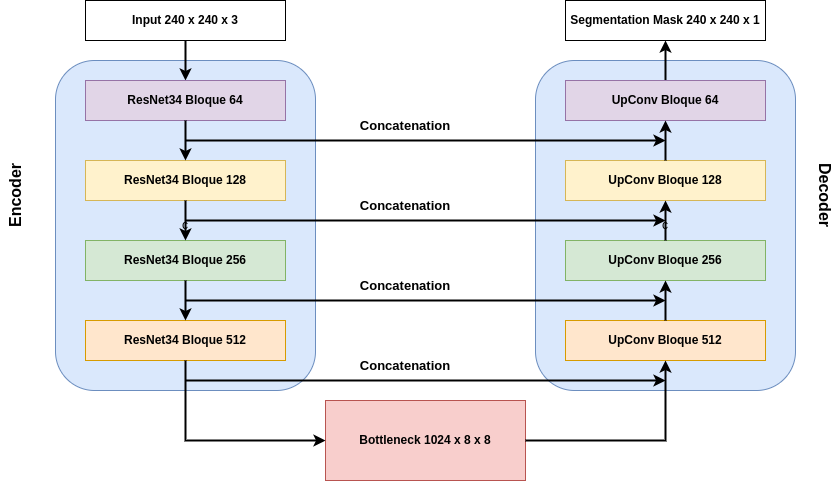
\includegraphics[width=1.0\linewidth]{imagenes/arquitectura_segmentacion.png}
	\caption{Arquitectura para la tarea de segmentación}
\end{figure}

Podemos ver como representamos a las skip connections como una simple concatenación de igual que forma que pasaba en las conexiones residuales pero de forma más general concatenando la salida de un módulo (grupo de capas) con la entrada de este.  


\section{Optimización de las arquitecturas}

En la siguiente sección detallaremos las funciones de pérdida usadas en cada arquitectura y la metodología seguida para llevar a cabo el entrenamiento de la red.

\subsection{Optimizador}

En este trabajo usaremos al optimizador por defecto de \textbf{Fastai}, \textbf{Adam}. El optimizador \textbf{Adam} (Adaptive Moment Estimation) \cite{kingma2014adam} es uno de los métodos de optimización más populares utilizados en el entrenamiento de redes neuronales profundas. Combina las ventajas de otros dos métodos conocidos: AdaGrad y RMSProp, ofreciendo una optimización más eficiente.

Adam ajusta los parámetros de la red neuronal basándose en el promedio de los gradientes y el promedio de los cuadrados de los gradientes. Los pasos principales que sigue son los siguientes:

\begin{enumerate}
	\item \textbf{Gradiente:} En cada iteración del entrenamiento, Adam calcula el gradiente de la función de pérdida con respecto a los parámetros del modelo. El gradiente indica la dirección y magnitud en la que los parámetros deben ajustarse para reducir la pérdida.
	
	\item \textbf{Promedio de gradientes (primer momento):} Adam calcula un promedio móvil de los gradientes. Esto ayuda a suavizar los cambios bruscos en la dirección del gradiente, proporcionando una dirección más estable para la actualización de los parámetros.

	$$ m_t = \beta_1 m_{t-1} + (1 - \beta_1) g_t $$

	donde $m_t$ es el promedio móvil de primer momento, $g_t$ es el gradiente en el tiempo $t$, y $\beta_1$ es el coeficiente de decaimiento exponencial para los promedios de primer momento.
	
	\item \textbf{Promedio de cuadrados de gradientes (segundo momento):} Adam también calcula un promedio móvil de los cuadrados de los gradientes. Esto permite ajustar la tasa de aprendizaje para cada parámetro individualmente, reduciendo la tasa de aprendizaje para los parámetros con gradientes grandes y aumentando la tasa para los parámetros con gradientes pequeños.

	$$ v_t = \beta_2 v_{t-1} + (1 - \beta_2) g_t^2 $$

	donde $v_t$ es el promedio móvil de segundo momento, $g_t$ es el gradiente en el tiempo $t$, y $\beta_2$ es el coeficiente de decaimiento exponencial para los promedios de segundo momento.
	
	\item \textbf{Corrección de sesgo:} Al principio del entrenamiento, los promedios móviles pueden estar sesgados hacia cero. Adam corrige este sesgo para obtener estimaciones más precisas de los promedios.

	$$ \hat{m}_t = \frac{m_t}{1 - \beta_1^t} $$

	$$ \hat{v}_t = \frac{v_t}{1 - \beta_2^t} $$

	
	\item \textbf{Actualización de parámetros:} Finalmente, Adam ajusta los parámetros del modelo utilizando los promedios móviles corregidos.

	$$ \theta_t = \theta_{t-1} - \frac{\alpha \hat{m}_t}{\sqrt{\hat{v}_t} + \epsilon} $$

	donde $\theta_t$ son los parámetros del modelo en el tiempo $t$, $\alpha$ es la tasa de aprendizaje, y $\epsilon$ es un pequeño valor para evitar la división por cero.
\end{enumerate}

\subsection{Funciones de pérdida}

En este apartado detallamos las funciones de pérdida utilizadas en las diferentes tareas.

\subsubsection{Función de pérdida para la reconstrucción de imágenes}

Usamos el \textbf{error absoluto medio} (MAE) de los píxeles de salida reconstruidos y los verdaderos como función de pérdida para realizar la reconstrucción de las imágenes. El MAE mide la magnitud promedio de las diferencias absolutas entre los valores predichos por el modelo y los valores reales. Esta métrica es útil para evaluar la precisión de la reconstrucción de las imágenes, ya que considera todas las diferencias de manera uniforme, sin penalizar más las diferencias grandes que las pequeñas.

$$ \text{MAE} = \frac{1}{n} \sum_{i=1}^{n} \left| y_i - \hat{y}_i \right| $$ 

Donde $n$ es el número total de píxeles en la imagen, $y_i$ es el valor verdadero del píxel $i$ y $\hat{y}_i$ es el valor reconstruido o predicho del píxel $i$.

En el contexto de la reconstrucción de imágenes, cada $y_i$ representa la intensidad del píxel en la imagen original, y cada $\hat{y}_i$ representa la intensidad del píxel en la imagen reconstruida por el modelo. El MAE proporciona una medida directa de cuán cerca están las intensidades de los píxeles reconstruidos de las intensidades reales.

También usaremos la misma pérdida como métrica de bondad de ajuste del modelo. Esto significa que, además de utilizar el MAE para optimizar el modelo durante el entrenamiento, también lo emplearemos para evaluar el desempeño del modelo en la reconstrucción de imágenes. Utilizar el MAE como métrica de evaluación nos permite tener una interpretación clara y consistente de cómo de bien se está desempeñando el modelo en términos de error promedio de los píxeles reconstruidos.

\subsubsection{Función de pérdida para clasificación}

Focal Loss es una función de pérdida que se ha demostrado ser particularmente efectiva para problemas de clasificación, especialmente en contextos donde hay un desequilibrio en las clases o cuando algunas muestras son más difíciles de clasificar que otras. Tras el procesamiento de datos, no existe un desbalanceo de datos grande. Sin embargo, la naturaleza de los tumores hacen que existan imágenes muy variables entre sí (con distinto grado de dificultad de optimización) es por ello que se opta por una pérdida que tenga algún mecanismo de control sobre esto. A continuación se explica por qué la Focal Loss puede ser mejor que la tradicional Cross Entropy Loss, especialmente en el contexto de datos con diferentes niveles de dificultad:

La Cross Entropy Loss es la función de pérdida estándar para problemas de clasificación y se define como:
$$  {\text{CE}} = - y_i \log(p_i) $$
$$  L_{\text{CE}} = - \sum_{i=1}^N y_i \log(p_i) $$

donde $y_i$ es la etiqueta verdadera y $p_i$ es la probabilidad predicha de la clase correcta. Aunque es efectiva, tiene algunas limitaciones:
\begin{enumerate}
	\item \textbf{Tratamiento Igualitario de todos los ejemplos}: Cross Entropy Loss trata todos los ejemplos de entrenamiento por igual, sin importar si son fáciles o difíciles de clasificar.
	\item \textbf{Sensibilidad al desbalanceo de clases}: No maneja bien los datos desbalanceados, donde algunas clases son mucho más frecuentes que otras.
\end{enumerate}

Focal Loss, propuesta por \cite{lin2017focal}, introduce un término adicional para enfocar el entrenamiento en ejemplos más difíciles. Se define como:

$$ {\text{FL}} = - \alpha (1 - p_t)^\gamma \log(p_t) $$
$$ L_{\text{FL}} = - \sum_{i=1}^N \alpha_t (1 - p_{t_i})^\gamma \log(p_{t_i})$$

donde $p_t$ es la probabilidad predicha de la clase correcta, $\alpha$ es un factor de ponderación para balancear la importancia de las clases, y $\gamma$ es el parámetro de focalización. Se puede desarrollar su principal ventaja:

\begin{enumerate}
	\item \textbf{Enfoque en ejemplos difíciles}: El término $(1 - p_t)^\gamma$ reduce la pérdida para los ejemplos bien clasificados (donde $p_t$ es alto) y mantiene alta la pérdida para los ejemplos mal clasificados (donde $p_t$ es bajo).
	
	\begin{enumerate}
		\item Cuando un ejemplo es fácil de clasificar ($p_t$ es alto), el término $(1 - p_t)^\gamma$ es pequeño, reduciendo su contribución a la pérdida total.
		\item Cuando un ejemplo es difícil de clasificar ($p_t$ es bajo), el término $(1 - p_t)^\gamma$ es grande, incrementando su contribución a la pérdida total.
	\end{enumerate}
	
	\item \textbf{Parámetro de Focalización}: El parámetro $\gamma$ ajusta el grado de focalización. Con $\gamma=0$, Focal Loss se reduce a la Cross Entropy Loss. Valores más altos de $\gamma$ incrementan el enfoque en los ejemplos difíciles.
	
	\item \textbf{Reducción del impacto de ejemplos fáciles}: Dado que los ejemplos fáciles no dominan el gradiente debido al término de focalización, el modelo no se sesga hacia las clases dominantes o los ejemplos que ya son bien clasificados.
	
\end{enumerate}

Esto implica los siguientes beneficios cuando existen datos de diferente dificultad.

\begin{enumerate}
	\item \textbf{Mejora del rendimiento general}: En muchos problemas de clasificación, hay ejemplos que son intrínsecamente difíciles de clasificar debido a la superposición de clases, ruido en los datos, o características ambiguas. Focal Loss ayuda a mejorar el rendimiento general del modelo al hacer que el modelo preste más atención a estos ejemplos difíciles durante el entrenamiento.
	
	\item \textbf{Mejor manejo de outliers}: Al reducir la contribución de ejemplos fáciles a la pérdida total, Focal Loss puede ayudar a mitigar el impacto de outliers o ejemplos atípicos que podrían desviar el modelo cuando se usa Cross Entropy Loss.
	
	\item \textbf{Robustez en modelos de gran escala}: En problemas similares como la detección de objetos en imágenes, donde el desequilibrio entre fondo y objeto puede ser significativo y algunos objetos son más difíciles de detectar que otros, Focal Loss ha demostrado ser particularmente útil.
	
\end{enumerate}

Focal Loss es una mejora sobre Cross Entropy Loss al proporcionar un mecanismo para enfocarse en ejemplos díficiles tales como imágenes donde los tumores sean pequeños. Con la gran en este problema de que realmente no queremos principalmente predecir muy bien la mayoría de ejemplos sino ser precisos en los ejemplos especialmente difíciles también para el personal médico. Por todo ello, se opta por utilizar \text{Focal Loss} para la primera tarea de clasificación.

\subsubsection{Función de pérdida para segmentación}

Como función de pérdida en segmentación se escoge el complemento negativo de su métrica más importante \textbf{similaridad Dice}: \textbf{Dice Loss}. Dice Loss se define como:

$$ L_{dice} = 1 - Dice(A, B) $$

Por lo tanto,  \textbf{Dice Loss} varía entre 0 y 1, donde 0 indica una superposición perfecta y 1 indica ninguna superposición (es decir, pérdida máxima).

Podemos enumerar las características que hacen de Dice Loss una de las pérdida más acertadas para la segmentación de tumores cerebrales. 

\begin{enumerate}
	\item \textbf{Sensibilidad a pequeñas áreas}: En la segmentación de tumores cerebrales, es crucial detectar incluso pequeñas regiones de tumores. El Dice Loss está diseñado para ser sensible a estas pequeñas áreas de superposición, lo que permite que el modelo se entrene para identificar y segmentar con precisión los bordes y áreas menos visibles del tumor.
	
	\item \textbf{Interpretabilidad clínica directa}: El coeficiente de similaridad Dice, en el que se basa el Dice Loss, proporciona una medida directa de cuán bien la predicción del modelo coincide con la realidad clínica. Esta métrica es intuitiva para los profesionales de la salud, ya que refleja la precisión de la segmentación en términos de superposición de áreas tumorales detectadas.
	
	\item \textbf{Robustez ante desbalanceo en la distribución de clases}: Los tumores cerebrales pueden representar solo una pequeña fracción de la imagen total, lo que genera desequilibrios en la distribución de clases. Dice Loss maneja este desequilibrio al penalizar menos la falta de predicción en áreas dominadas por el tejido cerebral normal, centrándose en mejorar la detección precisa de los tumores.
	
	\item \textbf{Optimización efectiva en el entrenamiento}: El uso de Dice Loss proporciona una superficie de optimización más suave y estable durante el entrenamiento de modelos de segmentación que otras pérdidas. Esto facilita la convergencia del modelo y reduce la necesidad de ajustes complejos de hiperparámetros, mejorando así la eficiencia del entrenamiento y la calidad de las segmentaciones obtenidas.
\end{enumerate}


\subsection{One-Cycle Policy}

La \textbf{política 1cycle} fue propuesta por \cite{smith2019super}, y es una técnica de programación de tasas de aprendizaje para mejorar el rendimiento del entrenamiento de redes neuronales. El objetivo principal es encontrar tasas de aprendizaje que aceleren el entrenamiento y mejoren la generalización del modelo. También ajusta la tasa de aprendizaje durante el entrenamiento de manera específica en función del número de iteraciones. Esta utiliza un ciclo de entrenamiento único en lugar de tasas de aprendizaje fijas durante todo el entrenamiento. Durante este ciclo, la tasa de aprendizaje varía de manera cíclica desde un valor inicial hasta un valor máximo y luego vuelve a descender.

En la primera mitad del ciclo, la tasa de aprendizaje aumenta gradualmente desde un valor inicial hasta un valor máximo. Este aumento permite una exploración más rápida del espacio de parámetros y puede ayudar a escapar de mínimos locales subóptimos. En la segunda mitad del ciclo, la tasa de aprendizaje disminuye gradualmente desde el valor máximo hasta el valor inicial. Esto permite una refinación más precisa de los pesos del modelo y una convergencia más estable hacia el mínimo global.

Además de ajustar la tasa de aprendizaje, la política 1cycle también propone variar el \textbf{momentum} (una técnica que ayuda a acelerar el entrenamiento). El momentum se incrementa en la fase de aumento y disminuye en la fase de descenso.

La política 1cycle también actúa como una forma de regularización. El uso de tasas de aprendizaje más altas en la fase de aumento y más bajas en la fase de descenso puede ayudar a prevenir el sobreajuste. También sugiere seleccionar los valores iniciales y máximos de la tasa de aprendizaje de manera específica. El valor máximo de la tasa de aprendizaje se elige típicamente como un valor que es varias veces mayor que el valor inicial. 

La duración total del ciclo puede variar, pero en general, se sugiere que sea aproximadamente igual al número total de épocas de entrenamiento.
La \textbf{política 1cycle} ha demostrado ser efectiva en mejorar la convergencia y la generalización en una variedad de tareas y arquitecturas de redes neuronales. Sin embargo, la selección precisa de los parámetros, como las tasas de aprendizaje inicial y máxima requiere ajustes específicos para cada objetivo y conjunto de datos.

En el uso conjunto de una política de \textbf{1cycle} y el optimizador \textbf{Adam} como se aplica en este trabajo, podemos entender como \textbf{1cycle} ajustaría la tasa de aprendizaje para una misma época (una tasa de aprendizaje global a una época) y Adam más tarde la refinaría ligeramente para cada ejemplo dentro de una época.  

En este trabajo usaremos esta política como forma de regularización y como método general para evitar la búsqueda de hiperparámetros manual para el proceso de aprendizaje. Para ello, en todo el trabajo sólo usaremos las llamadas a las funciones \texttt{fit\_one\_cycle()} para entrenar toda las capas de la red y \texttt{fine\_tune()} para cuando necesitemos diferenciar qué épocas entrenar toda la red (incluyendo la parte convolucional) o solo la parte densamente conectada. Ambas funciones son de la librería \textbf{Fastai} que implementan la política 1cycle. 

\section{Evaluación y métricas}

Para la evaluación se distinguirán entre tres subconjuntos de datos: entrenamiento, validación y test. Se utilizará un conjuntos fijos basado en \textbf{hold out}, común a todas las tareas. Por motivos de eficiencia no podemos permitirnos usar validación cruzada o distintos conjuntos variables. Estos conjuntos serán separados mediante la utilización de archivos CSV con las rutas absolutas de cada ejemplo para cada uno de ellos. 

Seguirán la siguiente distribución: un $49 \%$ para entrenamiento, $21 \%$ para validación y un $30 \%$ para test del conjunto total de datos (glioblastomas y meningiomas juntos) haciendo un reparto aleatorio entre ellos. Se sigue la regla de partición: $70 \%$ entrenamiento + validación y $30 \%$ test. La finalidad de cada subconjunto es para entrenamiento ajustar los modelos a este subconjunto de datos, el objetivo del conjunto de validación es elegir el mejor modelo de los probados, y el conjunto de test dar el resultado final garantizador de la bondad de los modelos.

\subsection{Métricas para clasificación}

Las métricas que vamos a usar para el proceso de clasificación son \textbf{accuracy balanceado} y \textbf{accuracy} que podremos calcular a través de la construcción de la matriz de confusión. 

\begin{enumerate}
	\item \textbf{Accuracy.} Mide cuántas predicciones del modelo son correctas respecto el total del predicciones. Se calcula como: 
	
	$$ \text{Accuracy} = \frac{\text{Nº de predicciones correctas}}{\text{Total de predicciones}} = \frac{TP + TN}{TP + TN + FP + FN}$$
	
	\item \textbf{Accuracy balanceado.} Esta métrica se usa en problemas de clasificación para manejar conjuntos de datos desbalanceados, donde las clases no están igualmente representadas. Se define como el promedio de las tasas de acierto (recall) obtenidas en cada clase, lo que ayuda a proporcionar una evaluación más justa y equilibrada del desempeño del modelo cuando las clases tienen diferentes tamaños.
	
	De forma general para un problema de clasificación de $N$ clases se calcula como:
	
	$$  \text{Balanced Accuracy} = \frac{1}{N} \sum_{i=1}^{N} \frac{TP_i}{TP_i + FN_i}$$
	
	De forma específica, para clasificación binaria $N = 2$ podemos expresarlo como:
	
	$$ \text{Balanced Accuracy} = \frac{1}{2} \left( \frac{TP}{TP + FN} + \frac{TN}{TN + FP} \right) $$ 
\end{enumerate}


\subsection{Métricas para segmentación}

Siguiendo la definición de evaluación de \textbf{BraTS} 2023, la evaluación de los tumores en su forma original comprende la segmentación de tres zonas diferenciadas según los tipos de tejidos que hay en ella. En \textbf{BraTS} se estudian los siguientes tres conjuntos de tejidos tumoral.

\begin{enumerate}
	\item \textbf{Enhancing Tumor ET}: Sólo incluye al tejido ET.
	\item \textbf{Tumor Core TC}: Incluye al tejido ET y al tejido NCR.
	\item \textbf{Whole Tumor WT}: Incluye a todos los tejidos enfermos: ET, NCR y ED. La segmentación de toda la lesión.
\end{enumerate}

Sin embargo, en este trabajo hacemos una reducción del problema por falta de recursos a \textbf{la segmentación únicamente del conjunto WT Whole Tumor}. De esta forma, la misión que tendremos es la de segmentar tejido enfermo o lesionado en todo el volumen de la resonancia. En otras palabras, diferenciar con la segmentación el tejido enfermo del tejido sano o la no existencia de tejido.

Para ello, se utilizará tres métricas. Las dos primeras utilizadas en todas las competiciones de \textbf{BraTS} y la tercera adicionalmente utilizada en los trabajos que han ido conformando el estado del arte como \cite{zhou2021latent}.

\begin{enumerate}
	\item \textbf{Similaridad Dice} : Mide la similaridad de dos conjuntos a través de la intersección de ambos respecto el tamaño total de los dos conjuntos.
	
	\begin{figure}[!h]
		\centering
		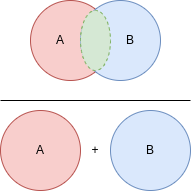
\includegraphics[width=0.25\linewidth]{imagenes/dicesimilarity.drawio.png}
		\caption{Interpretación del coeficiente de Similaridad Dice}
	\end{figure}
	
	Podemos expresarlo como:
	
	$$ Dice(A, B) = \frac{2 \times |A \cap B|}{|A| + |B|}$$
	
	Donde $A$ es la segmentación que proporcionará nuestro modelo y $B$ la verdadera.
	
	De forma más detallada, para una resonancia completa podemos expresarlo como:
	
	$$ Dice(A, B) =  2 \cdot \frac{\sum_{i=1}^{N} \sum_{j=1}^{C} A_{ij} B_{ij} + \epsilon}{\sum_{i=1}^{N} \sum_{j=1}^{C} A_{ij} + B_{ij} + \epsilon} $$ 
	
	Donde $N$ es el conjunto de todas las slices de la resonancia, $C$ el conjunto de clases en nuestro caso $C = 2$, $A_{ij}$ es el valor de la predicción en el pixel $i$ para clase $j$. $B_{ij}$ es el valor real en el pixel $i$ para la clase $j$. $\epsilon$ es una pequeña constante para evitar dividir entre 0. 
	
	\item \textbf{Distancia Hausdorff} : Esta métrica tiene el objetivo de medir geométricamente la mayor distancia resultado entre $A$ la predicción del modelo y la verdadera segmentación $B$, siendo $A$ y $B$, conjuntos de puntos o, píxeles.
	
	\begin{figure}[H]
		\centering
		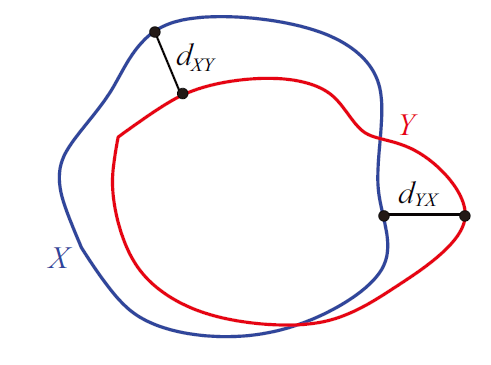
\includegraphics[width=0.4\linewidth]{imagenes/distanceHaussdorff.png}
		\caption{Distancias de Hausdorff entre dos conjuntos}
	\end{figure}
	
	Podemos enunciar la distancia máxima de Hausdorff:
	
	$$ H(A, B) = \max \left\{ \max_{a \in A} \min_{b \in B} d(a, b), \max_{b \in B} \min_{a \in A} d(a, b) \right\} $$
	
	Donde $a, b$ son puntos concretos en los conjuntos, $d(a, b)$ la distancia euclidiana entre los dos puntos y $A, B$ los conjuntos de puntos.
	
	Obtendremos la distancia de Hausdorff media de todos los slices de cada resonancia:
	
	$$ \bar{H}(A, B) = \frac{1}{|N|} \sum_{s \in N} H(A, B) $$
	
	De esta forma, a menor distancia de Hausdorff la segmentación salida y real son geométricamente más parecidas.
	
	\item \textbf{Sensibilidad o Recall} : Mide la proporción de casos positivos que fueron correctamente identificados por el modelo. En otras palabras y para nuestro problema, mide cuánto la segmentación predicción coincide con la segmentación verdadera, cuantificado en porcentaje.
	
	Podemos expresarlo como:
	
	$$ \text{Recall} = \frac{\text{TP}}{\text{TP} + \text{FN}} $$
	
	Donde $TP$ son los pixeles que son verdaderos positivos y $FN$ los pixeles que son falsos negativos.
	
\end{enumerate}

\section{Desarrollo para la predicción de la evolución}

Por falta de datos y recursos no pudimos entrar a resolver la predicción de la evolución de una lesión tumoral. Sin embargo, al menos teóricamente planteamos resolver esta tercera tarea. Es necesario tener en cuenta que la solución que aportaremos se sustenta en justo lo que no tuvimos, \textbf{más imágenes de una misma resonancia en diferentes momentos en el tiempo}. Se cree que la existencia de estos datos es una condición necesaria, ya que hasta el conocimiento que se tiene en este trabajo soluciones sin etiquetas no son viables.

Para construir una solución a este problema podemos valernos del \textbf{mismo encoder $g_{\phi}$ y representación latente $z$} utilizados en todas las arquitecturas con anterioridad. Posteriormente, podemos conectar un \textbf{Visual Transformer} que tenga como entrada la salida aplanada de la representación latente y tenga como output la segmentación en una instancia a corto plazo futura.

El objetivo del uso de una arquitectura transformadora es encontrar la correlación entre las \textbf{palabras} de entrada del decodificador (patches o píxeles de las imágenes) para poder minar \textbf{(si existen)} detalles en la imagen que lleven a poder predecir en el corto plazo cómo se extendería la lesión tumoral.

A continuación, podemos ver el esquema de este modelo hipótesis planteado.

\begin{figure}[H]
	\centering
	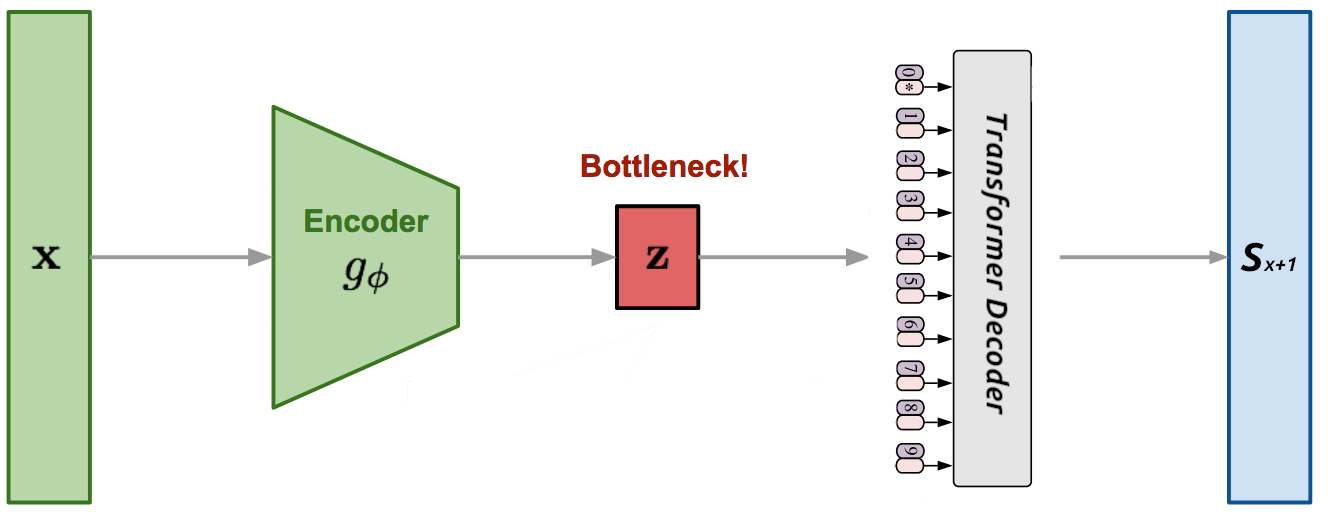
\includegraphics[width=0.9\linewidth]{imagenes/esquema_evolucion.png}
	\caption{Arquitectura propuesta para predicción de la evolución de los tumores}
\end{figure}

A continuación, hacemos algunas consideraciones de cómo llevar a cabo la optimización de esta arquitectura y detalles para poder llevarlo a la práctica.

\begin{enumerate}
	\item \textbf{Sigue siendo un problema de segmentación}. En la formulación del problema que estamos dando no estaríamos reconstruyendo la imagen futura sino su segmentación. Por lo tanto, pérdidas como \textbf{Dice Loss} seguirían siendo prometedoras.
	\item \textbf{Discretización del tiempo}. El tiempo es una magnitud que de forma precisa es discretizada en intervalos muy pequeños, por ejemplo podría ser discretizada en horas o minutos. En este problema carece de sentido una discretización demasiado precisa porque justamente lo interesante es ver las diferencias con la segmentación original para adelantarse a ellas. Un buen intervalo de discretización antes de entrenar el modelo y con datos en este intervalo son necesarios.
\end{enumerate}